%20130920 Work to be done still: data, conclusion appendices
%20130916 JW, first writing
\documentclass[iop]{emulateapj}

\usepackage{graphicx}
\usepackage{float}
\usepackage{amsmath,amsthm,amssymb}

\def\g{$g$}
\def\t{$t$}
\def\T{$T$}
\def\Ttwen{$T_{20}$}
\def\fillin{\#\#\#\#????}
\def\deg{^{\circ}}

\begin{document}

\title{Humpty Dumpty Had a Great Fall: Measuring the Acceleration due to Gravity with a Simple Pendulum}

\author{ Anthony D. Garcia
and
Joshua J. Wallace}
\affil{Advanced Undergraduate Lab, Department of Physics and Astronomy, University of Utah,
 115 South 1400 East, Salt Lake City, UT 84112
}

\begin{abstract}

\g man, \g!

\end{abstract}

\section{Introduction}

Of the four fundamental forces of nature, gravity is the one that we have the 
most experience with in our everyday lives.  It is such a constant in our lives 
that every movement we make factors in the force of gravity, even if we are not
aware of it. We put objects down, expecting them to stay there because of 
gravity. A basketball player shoots a ball upwards, expecting the familiar 
parabolic arc due to gravity to bring it back down into the basket.  Even the
common phenomenon known as walking relies on gravity's pull to give our feet
the friction needed to push us forward. Our experience with gravity is so
intimate that we can predict the exact trajectory of free-falling objects 
without having to use any equations or numbers (take the basketball player's 
shot for example. Shots are made regularly without any prior knowledge of 
the equations governing the motion of the ball).

One measure of the force of gravity is \g, the acceleration due to gravity. 
Since the acceleration due to gravity is independent of an object's mass, 
this provides a universal measure of gravity's pull on everything.

More than affecting our everyday lives, \g\ is a parameter that is used 
for a variety of applications. For instance, in geophysics 
variations in \g\ can be used to determine the structure and density of the 
crust and upper mantle below a given area of the earth's surface \citet{Geo}.
Another application of \g\ is in pendulum clocks. Christiaan Huygens 
first invented the pendulum clock about 1656 \citet{Murin} and its fairly high 
degree of accuracy causes it to still be used in households today (though 
admittedly pendulum clocks have been almost completely replaced by more 
accurate time\-keeping devices).  \g\ is an important parameter in 
calculating how long the period of a pendulum swing will be (the eager reader 
can skip ahead to section~\ref{sec:theory} for details of this calculation).  
So, for a good 
portion of man's history, \g\ determined our perception and measure of time.

To calculate \g, we will use a pendulum setup quite similar to that of the
pendulum clocks mentioned above.  Such pendulum experiments have been 
performed for centuries, first starting with Galileo \citet{Murin}. 
Specifically, we will use an idealization of a pendulum referred to as the 
"simple pendulum." Section~\ref{sec:theory} will give a more thorough 
introduction to the physics and idealizations of the simple pendulum.  
Here we state the intended 
goals of our study of the motion of a simple pendulum:  (1) To be able to 
determine the value of \g, which as discussed above is an important parameter
for a variety of calculations; (2) to test a mathematical model (introduced in 
section~\ref{sec:theory}) of a physical system and compare the correspondence 
between the two and (3) use the process as an introduction into the sources of 
errors and their propagation to gain greater skills as a physicist-in-training. 
The experiment we will be performing is discussed in great detail by 
Nelson and Olsson. \citet{Nelson} 

\section{Theoretical Background}
\label{sec:theory}


Later gater...

Also talk about small angle approximation...


\begin{figure}[H]
\centering
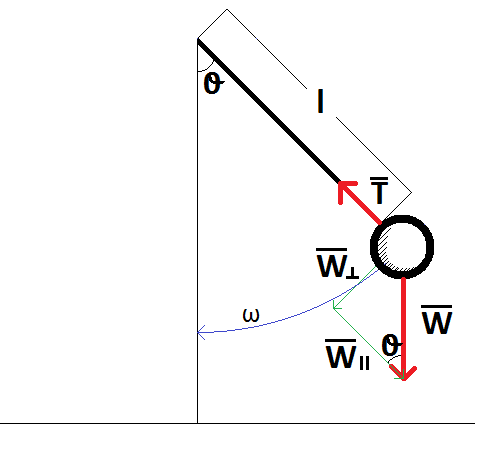
\includegraphics[width=85mm]{../../Images/FreebodyDiagram.png}
\caption{Diagram of a simple pendulum. 
$\theta$ is the angle between the string
and the rest position of the pendulum, $l$ is the length of the pendulum,
$\vec{W}$ is the weight force of the bob (i.e. $W = mg$), $\vec{W}_\perp$ is the 
component of the weight force perpendicular to $l$, $\vec{W}_\parallel$ 
is the component of the weight force parallel to $l$.}
\label{Pendulum}
\end{figure}


The motion of a simple pendulum can be derived by analyzing the torques (or forces) that acts 
on the bob of the pendulum. Assume the string that the pendulum hangs from is massless, and
its length l does not change. Friction on the string at the fulcrum as well as the
air drag on the bob is also ignored. See Appendix A for the full derivation
of the equation of motion for the simple harmonic oscillator.


From Figure 1; T is the tension force on the rope, l is the length of the
rope (or r$\cdot\hat{r}$, where $\hat{r}$ is a unit vector), $\theta$ is the angle, and W is the weight given by m$\cdot$g.


Using the small angle approximation
\begin{equation}
\boxed{sin\theta \approx \theta}
\end{equation}
for small angles, we derive the equation of motion
\begin{equation}
\boxed{T = 2\pi\sqrt{\frac{l}{g}}}
\end{equation}
to model a simple pendulum.
%%%%%%%%%%%%%%%%%%%%%%%%%%%%%%%%%%%%%%%%%%%%%%%%%%%%%%%%%%%%%%%



\section{Experimental Procedure}
\label{sec:procedure}

\subsection{Setup}

%%%%%%%%%%%%%%%%%%%%%%%%%%%%%%%%%%%%%%%%%%%%%%%%%%%%%%%%%%%%%%%%%


\begin{figure}[H]
\centering
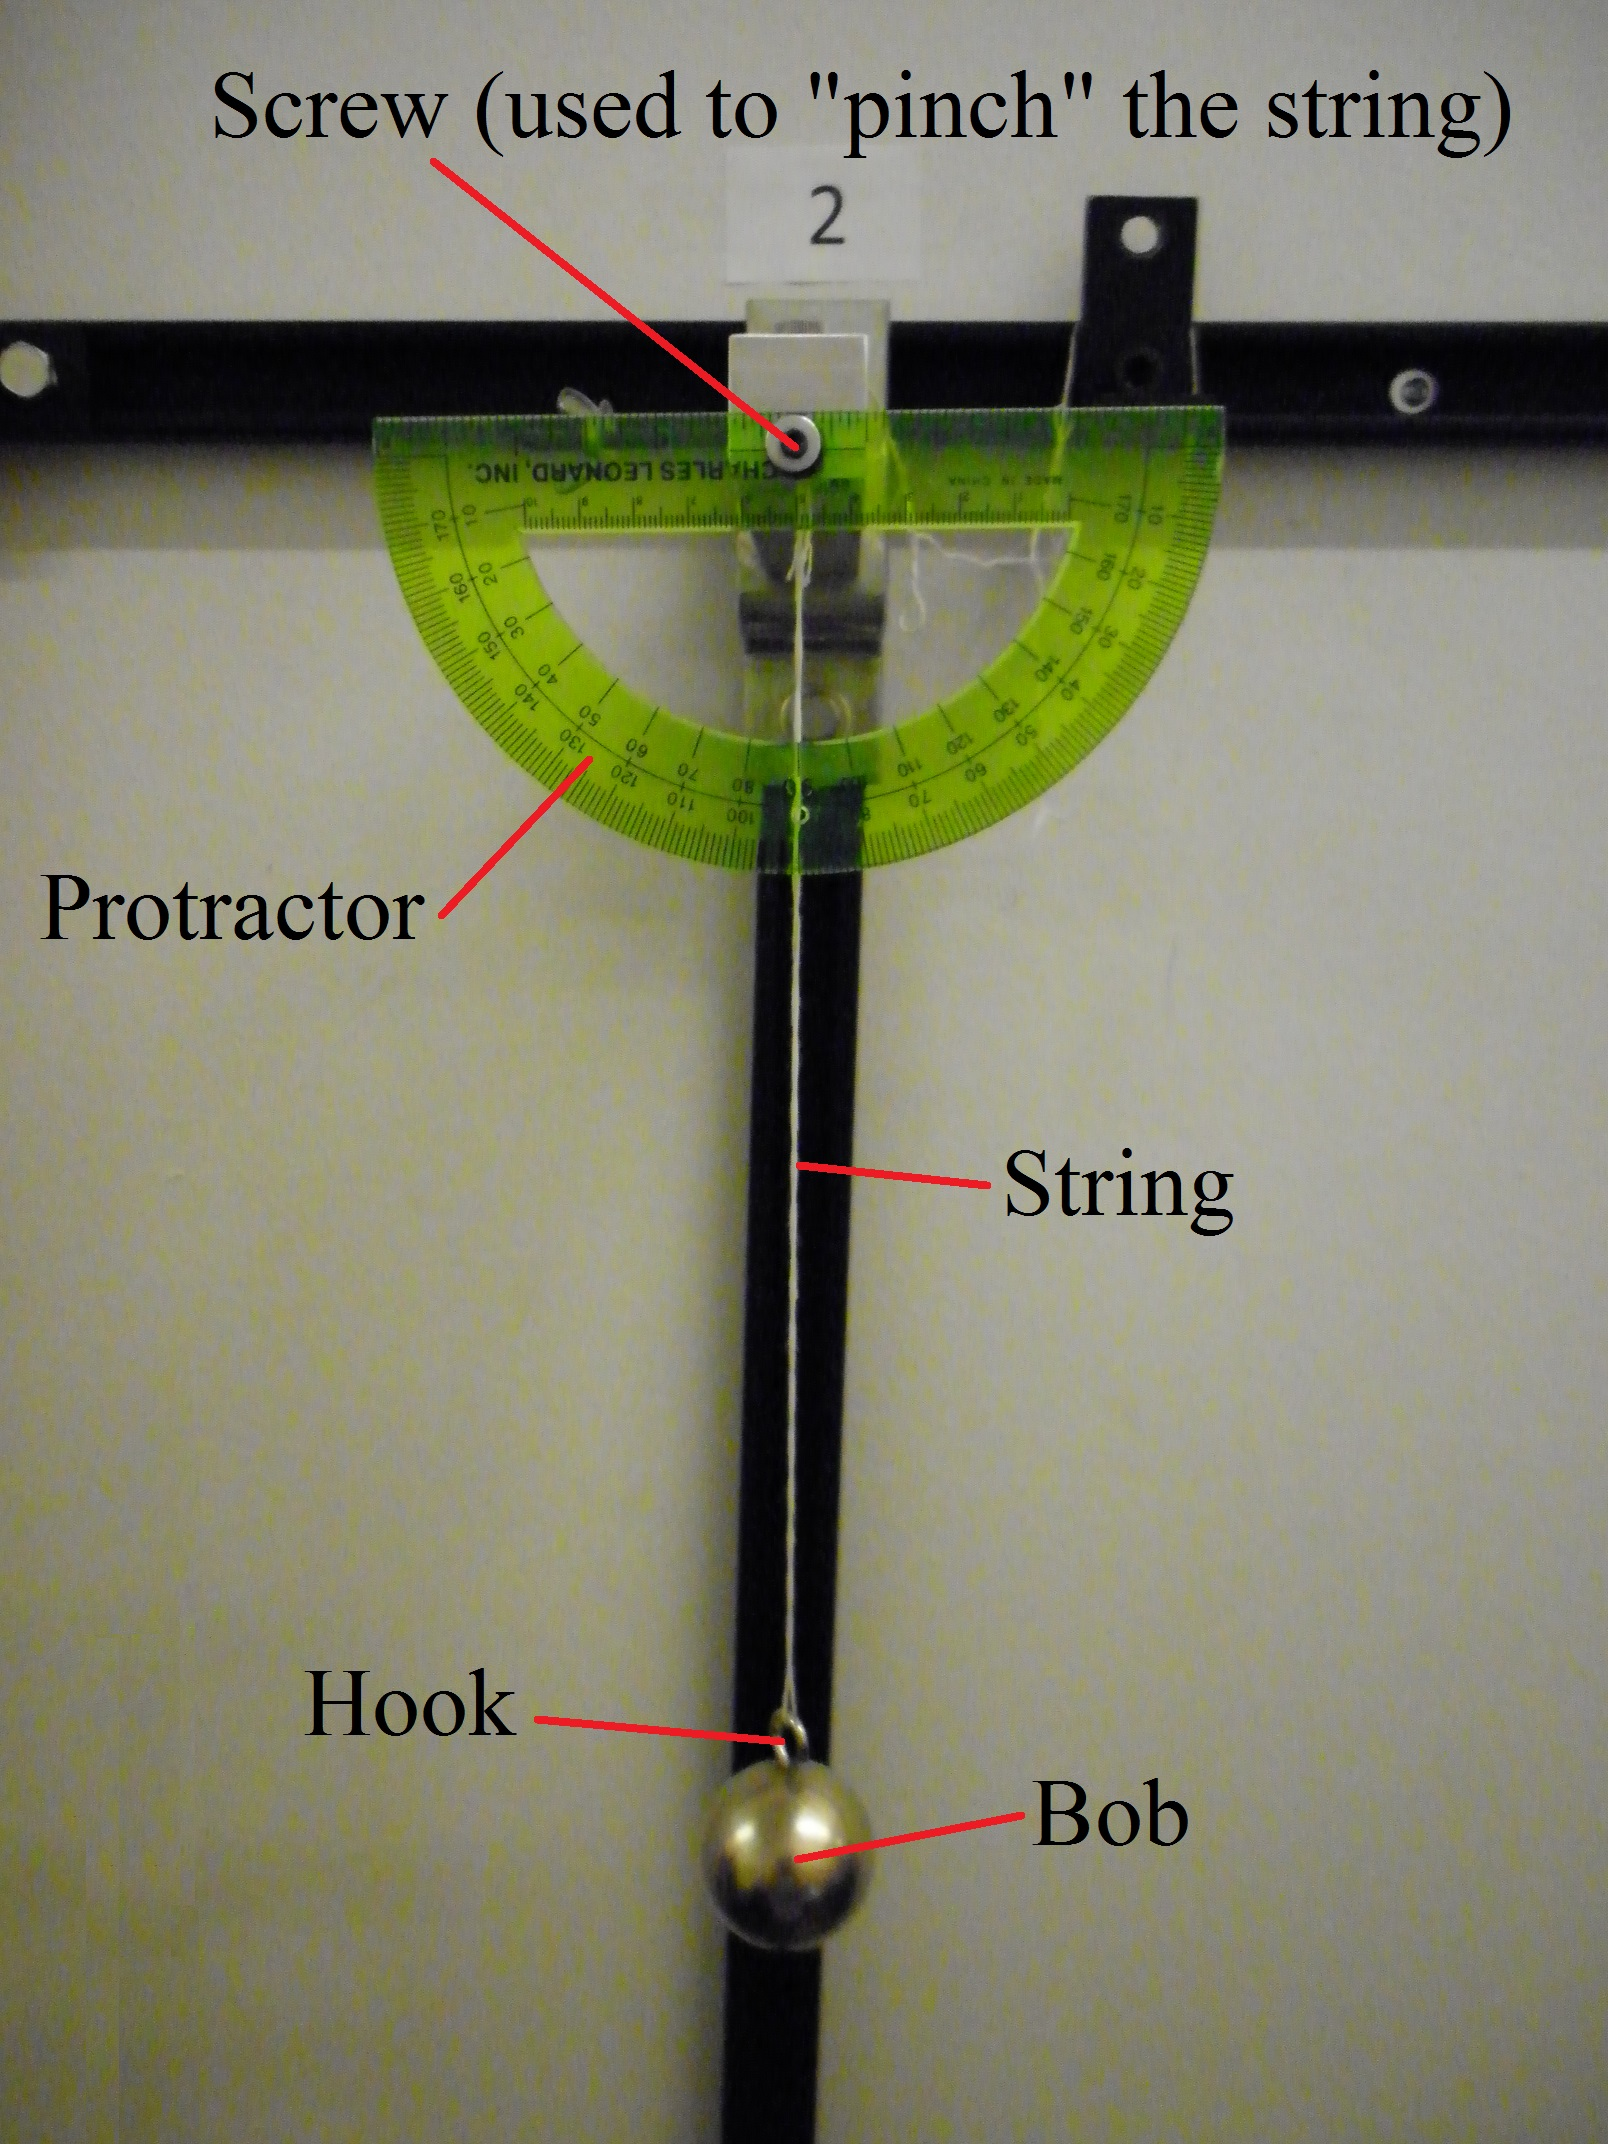
\includegraphics[width=85mm]{../../Images/Pendulum.JPG}
\caption{The bob is hung from the string by its hook. A screw pinches the string to act as
the pendulum's fulcrum. We measured the angle of the initial period with the 
protractor.}
\label{Pendulum}
\end{figure}


%%%%%%%%%%%%%%%%%%%%%%%%%%%%%%%%%%%%%%%%%%%%%%%%%%%%%%%%%%%%%%%%%%

The setup consisted of a metal frame attached to a wall, a string, a 
protractor, and a metal 
ball.  The metal ball connected to the string via a hook on the ball, which 
hooked into a loop tied in the string.  The pivot point of the pendulum was 
set with the same screw that held the protractor on to the frame.  The screw 
could be tightened or loosened to ensure the string's being pinned at the 
pivot point without causing the string to be torn.  Here is one limitation of 
our experiment; had a bolt been used instead of a screw, the bolt could 
have been tightened more (relative to the screw) against the string without 
severing the string.  This would have led to a better set pivot point.  
Instead, the screw's severing properties prevented us from setting the 
pivot point as tightly as would be possible with a bolt and therefore the 
pivot point itself (set with a screw) had the possibility of not being set 
well and therefore moving (which is not accounted for in our model, where the 
pivot point is set).

The string was anchored 
on top of the metal frame by wrapping it around a screw and then pinning the 
string to the frame with a nut on the screw.  The string length was easily 
adjusted by loosening the nut, adjusting the string, and re-tightening the 
nut.  The string had to be threaded through a tiny hole in the frame near 
the pivot point. 
A screw and wing nut on the side of the frame provided a convenient hold 
for a measuring stick to measure the length of the pendulum.  The frame also 
had a flat area in the frame level with it, which was useful for a tape 
measure to rest against when making a measurement.  Both the measuring stick 
and measuring tape could measure lengths down to $.1~cm$ 
($1\times 10^{-3}~m$).  A vernier caliper was used to measure the dimensions 
of the ball; this could measure lengths down to $1\times 10^{-5}~m$. There 
were also mirrors that could be used to reduce parallax.



The protractor was held firmly but not tightly against the frame, which 
allowed it to be aligned with the vertical when the pendulum was at rest 
but also 
kept it in place during minor bumps.  While this helped us not to have to 
reset the protractor position frequently it also made it hard to accurately 
set the protractor in the first place. The firmness with which the protractor 
was held made it difficult to move the protractor through the small angles 
necessary to set the $0\deg$ point as exact as possible.  This increased the 
uncertainty in our angle measurements.

We used MyChron brand stopwatches to time the period of the pendulum 
swing.  The stopwatch options we utilized in this experiment were the 
"start/stop" option and the "reset" option. The stopwatch could measure time 
We used a Westclox brand atomic clock as our standard for real time 
to see how much our stopwatch's time varied from real time.

\subsection{Procedure}

The first measurements we made were those of the ball diameter and the length 
of the hook on the top of the ball.  Due to the size of 
the ball and the large uncertainty associated with measuring the full length 
from the pivot point to the ball center (the center of mass of the
ball) we decided it would be best to measure the length of the string from the
pivot point to the top of the hook of the ball and then add the measured values 
for the hook height and ball radius afterwards.  The uncertainties from the 
caliper measurements are small enough compared to the uncertainty in using 
either a measuring stick or a tape measure in determining the length of the
string that making three separate measurements like this do not create an 
unnecessarily large uncertainty in length.  As stated above, a tape measure 
and/or measuring stick were used to measure the distance from the pivot point
to the top of the hook.  This was the distance that was measured when the
pendulum length was varied.

To reduce random error in measuring the pendulum length 
it is possible to measure the string length several 
different times and average the results; in practice, our different 
measurements returned either close to or exactly the same results, and so 
we adopted the practice of only measuring the length once. We also tried using 
mirrors to reduce parallax in the length measurement

The next step was to determine the uncertainty of the stopwatch we used. 
There were two sources of systematic 
uncertainty in the time measurements made by the stopwatch.  The first was the 
gain/lag the stopwatch had over real time.  The second was simply the finite 
gradations of time measured by the stopwatch ($.01 s$).  To account for the 
first source of systematic error (and also to determine which of the two 
authors were most accurate in their time measurements) we timed 
ourselves against an atomic clock for 1s and 100s intervals.  (On the second
day, 20s and 50s intervals). JW 
was determined to have the best accuracy {\bf (and precision?)} and was 
designated as the official timekeeper for the duration of the study.  
We then used the following equation to find how much the stopwatch time
differed from the atomic clock time (defined as $S$):

\begin{equation}
\label{eq:S}
S=\frac{t_{atomic}-t_{mean}}{t_{atomic}} 
\end{equation}

where $t_{atomic}$ is the real time as measured by the 
atomic clock 
and $t_{mean}$ is the mean of the times measured by the 
stopwatch.  This ratio was multiplied by all the \T\ we measured to give
the error from the gain/lag of the stopwatch.

Measuring against the atomic clock provided a measure of both the stopwatch's 
own limitations and the user's reaction time.  However, it is impossible to 
separate the two.  In order to fully account for the user's reaction time the 
above error was assumed to be due entirely to the stopwatch's limitations and 
a separate calculation was made of the timekeeper's reaction time.  This was 
done by having the timekeeper push the start and stop button on the 
stopwatch as fast as possible.  The average of these times was included in 
the overall error in measuring \T.

The next thing we did was determine the best way to measure the period of the 
pendulum's swing, i.e., a method that would allow us to both be accurate 
(allowing us to obtain a true value for \g) and precise (thus reducing random 
error). We first compared whether it was better to start timing a period from 
when the ball was released or to wait a period and start timing with the 
second period.  We wanted to see if there was a difference in accuracy and 
precision between the simultaneous double hand movement of releasing the ball 
while starting the stopwatch and just timing the period by eye. For this we 
timed a single swing of the pendulum eight times for both cases (i.e. starting 
timing with the swing and starting timing with the second swing). $\theta_{max}$ 
{\bf check thetamax!} was kept small (i.e., about $5\deg$) to ensure the 
validity of the small angle approximation (a more detailed analysis of what 
consitutes a "small angle" is provided in section \fillin). This was done 
for two different lengths: one around $26cm$ and the other around \fillin$cm$. 
$\theta_max$ {\bf check thetamax!} was kept small (i.e., about $5\deg$) 

Unfortunately the method with the lowest 
mean (timing from release) had the largest spread in times measured and 
vice-versa (for timing the second period). We chose to go 
with the method with the least uncertainty (i.e. lowest spread, or timing the 
second swing) over greatest accuracy because we figured that the method we 
used to determine the stopwatch gain/lag was closest to the method that timed 
the second swing; for both methods, the start and stop time were determined by 
eye.  If we had pushed a button on the atomic clock to start its timing at the 
same moment we had started the stopwatch, then this method would have been 
more similar to the method that used the release time of the pendulum to 
measure \T.  Therefore, the ratio $S$ determined by equation~\ref{eq:S} 
factors in the inaccuracy of the second period-measuring method more 
than the first method (in addition to the stopwatch's own gain/lag). The 
inaccuracy of the second method being thus accounted for we are free to choose 
the method that provides the lowest random uncertainty. 

We then measured the period of 20 oscillations (starting from the second 
swing) five separate times ($\theta_{max}$ was again kept around $5\deg$). 
We refer to this measurement as $T_{20}$. The purpose of this 
measurement was to reduce the error in determining the period.  Since 
$T=\frac{T_{20}}{20}$ it follows that
\begin{equation}
\label{eq:T20error}
\delta_T = \frac{\delta_{T20}}{20}.  Derive this later
\end{equation}
A more detailed derivation of equation~\ref{eq:T20error} is available in 
Appendix B ({\bf Provide more specific equation number in appendix!!}).
Thus, measuring 20 periods allows us to reduce the error in \T\ by a factor of 
20.  Since measuring 20 periods is not more difficult or significantly more 
time consuming than just measuring one period, this provides a relatively easy 
way to reduce the uncertainty in \T.  ?After measuring \Ttwen\ five times we 
found the mean, the standard deviation, ???and the standard deviation of the 
mean?.  As will be shown in section~\ref{sec:data}, five was a good number of trials to 
choose to reduce the random uncertainty to values comparable to the systematic 
uncertainties without having to perform the experiment and unnecessarily large 
number of times. {\bf We must show this!!!!}  The length of the string was 
then increased to the previous mentioned second length of 
about \fillin $cm$ and the above process was repeated (i.e., 
timing the first period, timing the second period, timing 20 periods).

A value for \g\ was then calculated for each of the above measurements (6 in 
total). Each was compared to the accepted value of \g, \fillin.  {\bf The 
method with the least uncertainty in \g\ was taken to be our method of choice 
in determining a more accurate value of \g\ later.}  The method chosen was the 
"\Ttwen\" method, where the time of 20 periods are measured and the value of 
\T\ is found by dividing \Ttwen\ by 20.  As shown in 
equation~\ref{eq:T20error} the error of \Ttwen\ is also divided by 20, thus 
causing this method to lead to greater precision.  {\bf hopefully it will lead 
to greater accuracy as well.  We must find out}. 

To minimize the uncertainty in measuring the string length, we used two 
different measuring methods to see which we felt gave us the most accuracy. 
We used a measuring stick and a tape measure.  We felt the tape measure gave 
us the most accurate measurement because we could put the $0cm$ end right at 
the pivot point (as opposed to the measuring stick, which required us to line 
up the stick with the pivot point level, adding in uncertainty, and also 
required us to reset it every time we wanted to make a measurement since it 
was in the way of the ball swing. The tape measure had this same situation 
as well, but since we could place its end directly on the pivot point level 
we knew we would have the same zero point every time. Thus, any error in 
measuring the zero point with the tape measure would be the same for all 
length measurements made by the measuring stick.  Since \g\ will be found 
from the slope of equation~\fillin, an error that is the same for all length 
measurements will not affect the calculated value of \g.  The measuring stick, 
on the other hand, would have to have its zero point reset for every length 
measure, thus providing random error in the length measurements that would 
not be the same for every length measurement and could affect the calculated 
value of \g).  It is important to note that the measuring tape's metal claw 
moves depending on whether you are measuring inside or outside and object. 
Since we were measuring inside an object (i.e., underneath the metal frame 
where the pivot point was located) we made sure that the metal claw was always 
pushed down towards the measuring tape to give us an accurate measure.  
Another reason the tape measure was chosen over the measuring stick was 
because it allowed us a more accurate measure at the ball's end of the string. 
Since the ball had a finite size, it got in the way of a direct measure of the 
top of the hook's location ("direct" meaning being able to lay the hook on the 
measuring stick and seeing which line it matched). {\bf include?:  We also could not rotate 
the ball out of the way of the measuring stick, since doing so required us to 
take a part of the ball's weight into our hand.  The problem with this was 
that the string we used was not truly inextensible as is ideal and the weight 
of the ball had an effect on the length of the string.  Taking the weight of 
the ball off the string and into our hand caused the string to relax from its 
fully extended length (how accurate can we determine this?}  The measuring 
tape, on the other hand, provided the flexibility necessary to bend the 
measuring device around the ball, allowing us to get a direct measure of the 
length (great care was taken to ensure that portion of the tape measure that 
was bent was past the portion of the tape measure involved in measuring the 
length so that the measurement was as accurate as possible). For long lengths 
of the string it became necessary for two people to operate the tape measure:
one to read the measurement at the bottom of the tape measure and one to hold 
claw next to the pivot point.  Care was taken that the claw was pushed down 
towards the measuring tape as described above.  Statisitical information was 
also obtained on the length of the pendulum by having each measured twice
......%We didn't measure everthing twice, and Yanil said we didn't need 
%to, I think so maybe shouldn't include this part.

Parallax...
%Still don't know how to use it...

We next tested the limits of validity for the small angle approximation and 
the accuracy of the model expressed by equation~\fillin. %large angle model
For three different lengths we measured \Ttwen\ for $\theta_{max} = 3\deg, 
5\deg, 10\deg, 20\deg,$ and $40\deg$.  %From these measurements it would seem 
%that $\theta_{max}\leq 10\deg$
After verifying the model of equation~\fillin\ we calculated that 
%This fillin corresponds to the model given in the handout
$\theta_{max}=5\deg$ will give us a model uncertainty small enough compared 
to our systematic uncertainties to be negligible.  See Appendix B section 
\fillin\ for a more detailed analysis.
%This section will be our calculation of T_err less than .1 percent
%should get theta_max=7.2.  5 degrees is within our error of 7.2.

Having established all our systematic uncertainties and determining the best 
method to measure \T for the resources we had, we then turned to making a more 
accurate measurement of \g.  To do this, we chose ten lengths in range from 
$~.3m$ to $~1.5m$.  Since we had recently discovered an easier way to use the 
measuring stick to make length measurements, each length was measured with 
both the tape measure and the measuring stick.  Since the measuring stick 
still proved hard to use to make accurate measurements and to keep continuity 
with our previous length measurements, we decided to use the lengths measured 
with the tape measure in our final calculation of \g. We then measured 
\Ttwen\ five times for each length.  

One thing we learned in measuring \T\ (likewise \T20) was how to accurately 
determine what constituted the beginning and end of a period.  The best 
method we found was to concentrate on the classical turning points. {\bf 
Should we include this?  We don't have data to back this up.}

Anything else to discuss?  Pitfalls?










\section{Data and Results}
\label{sec:data}

%%%%%%%%%%%%%%%%%%%%%%%%%%%%%%%%%%%%%%%%%%%%%%%%%%%%%%%%%%%%%%%%


\begin{table}[H]
\caption{Atomic Clock Measurements} % title of Table
\centering % used for centering table
\begin{tabular}{c c} % centered columns (4 columns)
\hline\hline %inserts double horizontal lines
Time Lapse & Stop Watch Time (s) \\ [0.5ex] % inserts table
%heading
\hline % inserts single horizontal line
50s & 49.85 \\ % inserting body of the table
    & 49.99 \\
    & 50.05 \\
    & 50.09 \\
    & 49.98 \\
$\overline{At}$ & 49.99 \\
$\sigma_{\overline{At}}$ & 0.04 \\    [1ex] % [1ex] adds vertical space
\hline %inserts single line
\end{tabular}
\label{table:nonlin} % is used to refer this table in the text
\end{table}


\begin{table}[H]
\caption{Reaction Time} % title of Table
\centering % used for centering table
\begin{tabular}{c c} % centered columns (4 columns)
\hline\hline %inserts double horizontal lines
& Stop Watch Reaction Time (s) \\ [0.5ex] % inserts table
%heading
\hline % inserts single horizontal line
& 0.15 \\ % inserting body of the table
& 0.13\\
& 0.15\\
& 0.14\\
& 0.17\\
$\overline{Rt}$ & 0.15 \\
$\sigma_{\overline{Rt}}$ & 0.01 \\    [1ex] % [1ex] adds vertical space
\hline %inserts single line
\end{tabular}
\label{table:nonlin} % is used to refer this table in the text
\end{table}




\begin{table}[H]
\caption{Period Measurement for Varying Lengths} %title of the table
\centering % centering table
\begin{tabular}{c rrrrr c} % creating eight columns
\hline\hline %inserting double-line
Length (m) & \multicolumn{5}{c}{$T_{20}$ (s)} & $\overline{T^2}$ ($s^2$)\\ [0.5ex]
\hline % inserts single-line
0.280 & 22.68 & 22.64 & 22.64 & 22.58 & 22.56 & 6.19\\ % Entering row contents
0.415 & 27.03 & 27.05 & 27.07 & 27.03 & 27.06 & 5.78\\
0.546 & 30.61 & 30.74 & 30.57 & 30.65 & 30.58 & 5.37\\
0.638 & 32.97 & 33.04 & 33.05 & 33.03 & 32.96 & 4.75\\
0.800 & 36.70 & 36.65 & 36.73 & 36.74 & 36.71 & 4.13\\
0.989 & 40.65 & 40.73 & 40.62 & 40.62 & 40.72 & 3.37\\
1.143 & 43.60 & 43.61 & 43.59 & 43.56 & 43.53 & 2.72\\
1.293 & 46.33 & 46.46 & 46.40 & 46.26 & 46.29 & 2.34\\
1.395 & 48.01 & 48.06 & 48.12 & 48.17 & 48.09 & 1.83\\
1.498 & 49.77 & 49.82 & 49.81 & 49.72 & 49.70 & 1.28\\ [1ex] % [1ex] adds vertical space
\hline % inserts single-line
\end{tabular}
\label{tab:hresult}
\end{table}


\begin{table}[H]
\caption{Dimensions of the bob} %title of the table
\centering % centering table
\begin{tabular}{c c c} % creating eight columns
\hline\hline %inserting double-line
Quantity & Uncertainty in Measurment & Measured Value\\ [0.5ex]
\hline % inserts single-line
Mass (g) & $\pm$ 0.1 & 226.2\\ % Entering row contents
Diameter (mm) & $\pm$ 0.03 & 38.02\\
Radius (m) & $\pm$ 0.00002 & 0.01901\\
Hook Length (mm)& $\pm$ 0.03 & 11.95\\
Hook Length (m)& $\pm$ 0.00003 & 0.01195\\[1ex] % [1ex] adds vertical space
\hline % inserts single-line
\end{tabular}
\label{tab:hresult}
\end{table}


%%%%%%%%%%%%%%%%%%%%%%%%%%%%%%%%%%%%%%%%%%%%%%%%%%%%%%%%%%%%%%%%%











\section{Discussion}
\label{sec:discuss}

Coriolis force, moment of inertia, air friction...














\section{Conclusion}














\acknowledgments

We thank Lia Papadopolous and Zach Carson for helpful conversations and 
suggestions.  We also thank Zheng Zheng for help with typesetting the 
document.






\begin{thebibliography}{}

%\bibitem[
\bibitem[[1]]{Geo}
[1] F.A. Darbyshire, R.S. White, and K.F. Priestly, "Structure of the crust and uppermost mantle of Iceland from a combined seismic and gravity study," {\it Earth Planet. Sci. Lett.} {\bf 48} (3), 409 (2000).
\bibitem[[2]]{Murdin}
[2] P. Murdin, (2008). {\it Full Meridian of Glory: Perilous Adventures in the Competition to Measure the Earth}, 1st Ed. (Copernicus Books, New York, NY 2008), p. 41.
\bibitem[[3]]{Nelson}
[3] R.A. Nelson and M.G. Olsson, "The Pendulum-Rich Physics from a Simple System," {\it Am. J. Phys.} {\bf 54}, 112-121 (1986).
\bibitem[[4]]{nist}
[4] http://physics.nist.gov/cuu/Constants/index.html
\bibitem[[5]]{nasa}
[5] http://nssdc.gsfc.nasa.gov/planetary/factsheet/earthfact.html


\end{thebibliography}{}


%%%%%%%%%%%%%%%%%%%%%%%%%%%%%%%%%%%%%%%%%%%%%%%%%%%%%%%

\appendix
\numberwithin{equation}{section}
\section{Appendix A: Additional Data}


\appendix
\numberwithin{equation}{section}
\section{Appendix B: Derivations and Error Propagation}


The motion of a simple pendulum can be derived by analysing the torques (or forces) that acts 
on the bob of the pendulum. Assume the string that the pendulum hangs from is massless, and
its length l does not change. Friction on the string at the fulcrum as well as the
air drag on the bob is also ignored. The definition of torque is given by;
\begin{equation}
\boxed{\tau = \vec{r} \times \vec{F} \equiv |\vec{r}||\vec{F}|\hat{n}sin\theta}
\end{equation}
From Figure 1; T is the tension force on the rope, l is the length of the
rope (or r$\cdot\hat{r}$, where $\hat{r}$ is a unit vector), $\theta$ is the angle, and W is the weight given by m$\cdot$g.
Using the definition of the cross product;
\begin{align*}
\tau_T & = \vec{l} \times \vec{T} = 0 & \text{($\vec{l}$ is $||$ to $\vec{T}$)}\\
\tau_W & = \vec{l} \times \vec{W}\\
& = |\vec{l}||\vec{W}|\hat{n}sin\theta\\
& = -l\cdot W\cdot sin\theta & \text{($\hat{n}$ is "-")}\\
& = -l\cdot mg\cdot sin\theta & \text{(W = m$\cdot$g)}\\
\end{align*}
\begin{equation}
\boxed{\tau_W = -lmgsin\theta}
\end{equation}
Newton's second law applied to rotational motion is given by,
\begin{equation}
\tau = I\cdot\alpha
\end{equation}
where I is the moment of inertia. The simple pendulum will be 
treated as a point particle at a distance l from the origin.
Equating the two we get;
\begin{align*}
\tau_W = -lmgsin\theta & = I\cdot\alpha\\
& = (ml^2)\alpha & \text{(I = $ml^2$ for a point particle)}\\
& = (ml^2)\ddot{\theta} & \text{($\alpha = \ddot{\theta}$)}\\
\Rightarrow -gsin\theta & = l\ddot{\theta}\\
\Rightarrow l\ddot{\theta} + gsin\theta & = 0
\end{align*}
The Taylor series of sin($\theta$) is given by
\begin{equation}
\boxed{sin\theta = \theta - \frac{\theta^3}{3!} + \frac{\theta^5}{5!} - \frac{\theta^7}{7!} + \frac{\theta^9}{9!} - ...}
\end{equation}
For small angles we get
\begin{equation}
\boxed{sin\theta \approx \theta}
\end{equation}
which is the small angle approximation. Note that the small angle approximation 
is valid to about $15^{\circ}$.\\
Applying the small angle approximation to our equation of motion we get
\begin{align}
\boxed{l\ddot{\theta} + g\theta = 0}
\end{align}
Solving the the differential equation;
\begin{align*}
l\ddot{\theta} + g\theta & = 0\\
\Rightarrow \ddot{\theta} + \frac{g}{l}\theta & = 0\\
\end{align*}
The characteristic equation for this Differential Equation is
\begin{align*}
x^2 + \frac{g}{l} = 0\\
\Rightarrow x = \pm i\sqrt{\frac{g}{l}}
\end{align*}
Which has the general equation
\begin{align*}
\theta(t) & = C_1e^{i\sqrt{(g/l)}t} + C_2e^{-i\sqrt{(g/l)}t}\\
& = C_1[cos(\sqrt\frac{g}{l}t) + isin(\sqrt\frac{g}{l}t)] +\\ 
&~~~~~~+ C_2[cos(\sqrt\frac{g}{l}t) - isin(\sqrt\frac{g}{l}t)]\\
& = (C_1 + C_2)cos(\sqrt\frac{g}{l}t) + i(C_1 - C_2)sin(\sqrt\frac{g}{l}t)\\
& = Acos(\sqrt\frac{g}{l}t) + Bsin(\sqrt\frac{g}{l}t)\\
\end{align*}
If we create a right triangle with the constants A and B, to get a hypotenuse
constant C and angle $\phi$. That triangle can be describe with the terms;
\begin{align*}
sin\phi & = \frac{B}{C}\\
cos\phi & = \frac{A}{C}
\end{align*}
Then if we multiply the general solution by C/C;
\begin{align*}
\theta(t) & = C[\frac{A}{C}cos(\sqrt\frac{g}{l}t) + \frac{B}{C}sin(\sqrt\frac{g}{l}t)]\\
& = C[cos(\phi) cos(\sqrt\frac{g}{l}t) + sin(\phi)cos(\sqrt\frac{g}{l}t)]\\
& = C[cos(\phi) cos(\sqrt\frac{g}{l}t) - sin(-\phi)cos(\sqrt\frac{g}{l}t)]\\
& = C[cos(\sqrt\frac{g}{l}t - \phi)]
\end{align*}
$\phi$ is the phase shift. For the simple pendulum the phase shift is zero 
because the initial angle is $\theta_0$. This gives\\
\begin{equation*}
\theta(t) = Ccos(\sqrt\frac{g}{l}t)
\end{equation*}
Then for t = 0
\begin{align*}
\theta(0) & = C[cos(0)]\\
& = C\\
& \equiv \theta_0
\end{align*}
Then the solution to the equation of motion is
\begin{equation}
\boxed{\theta(t) = \theta_0[cos(\sqrt\frac{g}{l}t)]}
\end{equation}
We know that the derivative of $\theta(t)$ is $\omega$ (angular velocity)
\begin{align*}
\dot{\theta}(t) & = \omega(t)\\
& = -\sqrt\frac{g}{l}\theta_0[sin(\sqrt\frac{g}{l}t)]
\end{align*}
Angular velocity is zero every time it reaches the max height during an oscillation. We can than see for
for what times this occurs by setting $\omega \equiv 0$.
\begin{align*}
\omega & \equiv 0\\
-\sqrt\frac{g}{l}\theta_0[sin(\sqrt\frac{g}{l}t_n)] & = 0\\
\Rightarrow \sqrt\frac{g}{l}t_n & = sin^{-1}(0)\\
& = 2\pi n\\
\Rightarrow t_n & = 2\pi n\sqrt\frac{l}{g}
\end{align*}
This periodicity is what we call the Period;
\begin{equation}
\boxed{T = 2\pi \sqrt\frac{l}{g}}
\end{equation}
%%%%%%%%%%%%%%%%%%%%%%%%%%%%%%%%%%%%%%%%%%%%%%%%%%%%%%%%%






\end{document}
